\section{Experiments and Analysis}

\subsection{Experimental Setup}
\textbf{Benchmarks:} To evaluate ReSum's effectiveness in overcoming context limitations for complex queries, we conduct experiments on three challenging benchmarks where agents typically require extensive exploration: \textbf{GAIA}~\citep{mialon2023gaia}, \textbf{BrowseComp}~\citep{bc_en}, and its Chinese counterpart \textbf{BrowseComp-zh}~\citep{bc_zh}. For GAIA, we follow existing works by using the 103-sample text-only validation subset. We exclude simpler benchmarks such as SimpleQA~\citep{wei2024simpleqa}, WebWalkerQA~\citep{wu2025webwalker}, and xBench-DeepSearch~\citep{xbench}, where most cases can be resolved within standard context limits, rendering the ReAct paradigm more suitable.

\textbf{Evaluation:} Following standard practice in web agent research~\citep{gao2025asearcher, dong2025arpo}, we consistently use Qwen2.5-72B-Instruct as the scoring model to assess whether the predicted answer aligns with the ground truth (see Appendix~\ref{appendix:llm-as-judge} for justification). Specifically, we report the average \textbf{Pass@1} over all test samples, as well as \textbf{Pass@3} across three rollouts for each sample. Unless otherwise stated, we set the maximum tool call budget to 60 for all inference paradigms to ensure a fair comparison.
% TODO: 是否需要强调rationale for LLM-as-Judge? 

\textbf{Baselines \& Implementations:} We assess ReSum's effectiveness under two settings: \textbf{training-free} and \textbf{training-required}. In the training-free setting, we apply ReSum directly to off-the-shelf agents, comparing it against \textbf{ReAct} and \textbf{Recent History}, i.e., truncating history to the latest 22$k$ tokens when approaching the context limit. We also compare with \textbf{MEM1}~\citep{zhou2025mem1}, a representative context management method. In the training-required setting, we evaluate whether RL optimization enhances paradigm mastery. We 
compare ReSum-GRPO against standard GRPO and MEM1-GRPO. For ReSum inference, summarization is consistently triggered as the conversation history approaches the context limit, and leverages ReSumTool-30B for summarization unless specifically stated. Further implementation details are provided in Appendix~\ref{appendix:implementation}.
% with the standard GRPO algorithm. Specifically, we evaluate both ReSum and ReAct paradigms on different RL-trained web agents to check whether ReSum-GRPO enhances the agents' proficiency with ReSum. For ReSum inference, summarization is consistently triggered as the conversation history approaches the context limit, and leverages ReSumTool-30B unless specifically stated. Additionally, we include a comparison with \textbf{MEM1}~\citep{zhou2025mem1}, a representative context management method under both settings.

\textbf{Choice of Web Agents:} We conduct experiments on open-source web agents of varying scales to ensure a comprehensive evaluation, including \textbf{WebSailor-3B}\footnote{\href{https://huggingface.co/Alibaba-NLP/WebSailor-3B}{https://huggingface.co/Alibaba-NLP/WebSailor-3B}}, \textbf{WebSailor-7B}\footnote{\href{https://huggingface.co/Alibaba-NLP/WebSailor-7B}{https://huggingface.co/Alibaba-NLP/WebSailor-7B}}, and \textbf{WebSailor-30B-A3B}\footnote{This is a reproduced version using the same training data as the WebSailor series, with rejection fine-tuning (RFT) applied to Qwen3-30B-A3B-Base model for 2 epochs.}. Note that all these agents are constrained by a 32$k$ token context limit.

\definecolor{ours}{HTML}{E6F0FF}

\begin{table*}[!t]
    \centering
    \caption{\textbf{Performance comparison (in \%) between paradigms under training-free settings.} \textbf{MEM1} is evaluated exclusively on WebSailor-30B due to the limited instruction-following capabilities of smaller backbones to suit such a paradigm. \colorbox{ours}{Blue} indicates results using ReSum with our developed ReSumTool-30B, which consistently outperforms baselines. \textbf{Bold} highlights the best results for each backbone agent. Results with $^{\dag}$ are sourced from \cite{liu2025webexplorer}, representing leading pre-trained models paired with search and visit tools to illustrate the datasets' performance landscape.}
    \resizebox{0.92\linewidth}{!}{
    \begin{tabular}{lll|cc|cc|cc}
         \toprule
         \rowcolor{COLOR_MEAN}  & & & \multicolumn{2}{c|}{\textbf{GAIA}} & \multicolumn{2}{c|}{\textbf{BrowseComp-zh}} & \multicolumn{2}{c}{\textbf{BrowseComp}}  \\
        \rowcolor{COLOR_MEAN} \multirow{-2}{*}{\textbf{Agent}} & \multirow{-2}{*}{\textbf{Paradigm}} & \multirow{-2}{*}{\textbf{Summary Tool}} & Pass@1 & Pass@3 & Pass@1 & Pass@3  & Pass@1 & Pass@3 \\ \midrule 
          Claude-4$^{\dag}$ & ReAct & $-$ & 68.3 & $-$ & 29.1 & $-$ & 12.2 & $-$ \\ 
          OpenAI-o3$^{\dag}$ & ReAct & $-$ & 70.5 & $-$ & 58.1 & $-$ & 50.9 & $-$ \\
        Kimi-K2$^{\dag}$ &  ReAct & $-$ &  57.7 & $-$ & 28.8 & $-$ & 14.1 & $-$ \\ 
        DeepSeek-v3.1$^{\dag}$ & ReAct & $-$ & 63.1 & $-$ & 49.2 & $-$ & 30.0 & $-$  \\ \midrule

        % \rotatebox{90}{\textbf{WebSailor-3B}}
        
        \multirow{7}{*}{\textbf{WebSailor-3B}} & ReAct & \multirow{2}{*}{$-$} & 25.6 & 42.7 & 8.2 & 17.0 & 3.3 & 5.6 \\ 
        & Recent History & & 27.2 & 44.7 & 13.2 & 24.3 & 3.8 & 8.9 \\ \cmidrule{2-9} 
        &  \multirow{5}{*}{ReSum} & Qwen3-30B & 27.5 & 45.6 & 6.9 & 14.5 & 4.2 & 7.8 \\
        & & \cellcolor{ours}{ReSumTool-30B} & \cellcolor{ours}{35.3} & \cellcolor{ours}{52.4} & \cellcolor{ours}{13.7} & \cellcolor{ours}{24.6} & \cellcolor{ours}{6.8} & \cellcolor{ours}{10.8} \\ 
        & & GPT-OSS-120B & \textbf{40.5} & \textbf{65.1} & \textbf{15.2} & \textbf{28.0} & \textbf{8.5} & \textbf{15.8} \\ 
        & & Qwen3-235B  & 32.4 & 49.5 & 11.1 & 23.9 & 5.7 & 10.3 \\ 
        & & DeepSeek-R1-671B  & 39.2 & 60.2 & 13.0 & 23.5 & 7.5 & 13.4 \\ \midrule
        
        \multirow{7}{*}{\textbf{WebSailor-7B}} & ReAct & \multirow{2}{*}{$-$} & 31.7 & 44.7 & 13.2 & 25.6 & 5.7 & 10.3 \\ 
        & Recent History & & 33.0 & 48.5 & 15.2 & 28.0 & 5.2 & 9.4 \\ \cmidrule{2-9}
        & \multirow{5}{*}{ReSum} & Qwen3-30B & 34.6 & 48.5 & 13.3 & 26.6 & 5.8 & 10.3 \\ 
        & & \cellcolor{ours}{ReSumTool-30B} & \cellcolor{ours}{40.5} & \cellcolor{ours}{60.2} & \cellcolor{ours}{17.2} & \cellcolor{ours}{30.8} & \cellcolor{ours}{9.0} & \cellcolor{ours}{15.2} \\ 
        & & GPT-OSS-120B & 42.4 & \textbf{61.2} & \textbf{19.2} & \textbf{35.6} & \textbf{10.5} & \textbf{17.2} \\ 
        & & Qwen3-235B & \textbf{43.4} & 60.2 & 18.1 & 32.9 & 8.7 & 15.2 \\
        & & DeepSeek-R1-671B & 41.1 & 58.3 & 17.1 & 32.2 & 10.3 & 16.6 \\ \midrule 

        \multirow{8}{*}{\textbf{WebSailor-30B}} & ReAct & \multirow{3}{*}{$-$} & 45.0 & 60.2 & 23.9 & 38.4 & 12.8 & 21.8 \\ 
        & Recent History & & 40.1 & 56.3 & 24.1 & 40.1 & 10.3 & 16.7 \\ 
        & MEM1 & & 33.3 & 52.4 & 25.0 & 41.2 & 12.7 & 22.5  \\ \cmidrule{2-9}  
        
        &  \multirow{5}{*}{ReSum} & Qwen3-30B & 45.6 & 61.2 & 24.8 & 40.1 & 12.2 & 20.4 \\
        & & \cellcolor{ours}{ReSumTool-30B} & \cellcolor{ours}{47.3} & \cellcolor{ours}{63.1} & \cellcolor{ours}{24.1} & \cellcolor{ours}{42.6} & \cellcolor{ours}{16.0} & \cellcolor{ours}{25.4} \\ 
        & & GPT-OSS-120B & \textbf{51.5} & 68.9 & \textbf{27.3} & \textbf{46.4} & \textbf{18.8} & \textbf{30.9} \\ 
        & & Qwen3-235B & 46.9 & 67.0 & 25.7 & 42.2 & 17.2 & 26.7 \\ 
        & & DeepSeek-R1-671B & 49.2 & \textbf{71.8} & 27.1 & 41.5 & 13.7 & 22.6 \\ 
       \bottomrule
    \end{tabular}
    }
    \label{tab:training_free_performance}
\end{table*}


\begin{table*}[!t]
    \centering
    \caption{\textbf{Performance comparison (in \%) between RL algorithms.} ReSum-GRPO enables agents to become better familiarized with the ReSum paradigm, boosting performance. Results with $^{\dag}$ are sourced from \cite{liu2025webexplorer}, representing powerful web agents trained with \textbf{10K+} samples.}
    \vspace*{-6pt}
    \resizebox{0.9\linewidth}{!}{
    \begin{tabular}{lll|cc|cc|cc}
         \toprule
         \rowcolor{COLOR_MEAN}  & & & \multicolumn{2}{c|}{\textbf{GAIA}} & \multicolumn{2}{c|}{\textbf{BrowseComp-zh}} & \multicolumn{2}{c}{\textbf{BrowseComp}}  \\
        \rowcolor{COLOR_MEAN} \multirow{-2}{*}{\textbf{Agent}} & \multirow{-2}{*}{\textbf{RL}} & \multirow{-2}{*}{\textbf{Paradigm}} & Pass@1 & Pass@3 & Pass@1 & Pass@3  & Pass@1 & Pass@3 \\ \midrule 
         Qwen3-ARPO-14B & ARPO & ReAct & 43.7 & $-$ & $-$ & $-$ & $-$ & $-$  \\
        MiroThinker-8B$^{\dag}_\text{v0.1}$ & DPO & ReAct & 46.6 & $-$ & 13.6 & $-$ & 8.7 & $-$ \\ 
        MiroThinker-32B$^{\dag}_\text{v0.1}$ & DPO & ReAct & 57.3 & $-$ & 17.0 & $-$ & 13.0 & $-$ \\ 
        ASearcher-QWQ-32B$^{\dag}$ & GRPO & ReAct & 52.8 & $-$ & 15.6 & $-$ & 5.2 & $-$ \\
        WebExplorer-8B$^{\dag}$ & GRPO & ReAct & 50.0 & $-$ & 32.0 & $-$ & 15.7 & $-$ \\
        DeepDive-32B & GRPO & ReAct & $-$ & $-$ & 29.7 & $-$ & 15.3 & $-$ \\
        
        \midrule

         \multirow{5}{*}{\textbf{WebSailor-3B}}
        & $-$ & ReAct & 25.6 & 42.7 & 8.2 & 17.0 & 3.3 & 5.6 \\  \cmidrule{2-9}
        & \multirow{2}{*}{GRPO} & ReAct & 28.5 & 48.5 & 11.8 & 22.5 & 4.2 & 8.5 \\
        & & ReSum & \textbf{38.5} & 53.4 & 17.3 & 29.1 & 8.5 & 13.0 \\ \cmidrule{2-9}
        & \cellcolor{blue!10} \textbf{ReSum-GRPO} & \cellcolor{blue!10}ReSum & \cellcolor{blue!10} 37.9 & \cellcolor{blue!10}\textbf{56.3} & \cellcolor{blue!10}\textbf{20.5} & \cellcolor{blue!10}\textbf{34.3} & \cellcolor{blue!10}\textbf{9.2} & \cellcolor{blue!10}\textbf{13.0} \\ \midrule

        \multirow{5}{*}{\textbf{WebSailor-7B}}
        & $-$ & ReAct & 31.7 & 44.7 & 13.2 & 25.6 & 5.7 & 10.3 \\  \cmidrule{2-9}
        & \multirow{2}{*}{GRPO} & ReAct & 34.0 & 47.6 & 18.7 & 31.8 & 5.8 & 10.0 \\
        & & ReSum & 37.2 & 53.4 & 25.4 & \textbf{40.8} & 8.5 & 15.0\\ \cmidrule{2-9}
        & \cellcolor{blue!10} \textbf{ReSum-GRPO} &
        \cellcolor{blue!10}ReSum & \cellcolor{blue!10}\textbf{42.4} & \cellcolor{blue!10}\textbf{60.2} & \cellcolor{blue!10}\textbf{27.1} & \cellcolor{blue!10}39.5 & \cellcolor{blue!10}\textbf{12.3} & \cellcolor{blue!10}\textbf{18.5} \\ \midrule

        \multirow{6}{*}{\textbf{WebSailor-30B}}
        & $-$ & ReAct & 45.0 & 60.2 & 23.9 & 38.4 & 12.8 & 21.8 \\  \cmidrule{2-9}
        & \multirow{2}{*}{GRPO} & ReAct & 48.2 & 62.1 & 23.3 & 36.7 & 14.3 & 21.5 \\ 
        & & ReSum & 48.5 & 61.2 & 29.3 & 42.6 & 15.0 & 25.0 \\ \cmidrule{2-9}
        & MEM1-GRPO & MEM1 & 35.7 & 54.4 & 29.1 & 45.0 & \textbf{19.5} & \textbf{29.7} \\ \cmidrule{2-9}
        & \cellcolor{blue!10} \textbf{ReSum-GRPO} & \cellcolor{blue!10}ReSum & \cellcolor{blue!10}\textbf{48.5} & \cellcolor{blue!10}\textbf{68.0} & \cellcolor{blue!10}\textbf{33.3} & \cellcolor{blue!10}\textbf{48.8} & \cellcolor{blue!10}18.3 & \cellcolor{blue!10}26.5 \\ 
       \bottomrule
    \end{tabular}
    }
    \label{tab:rl_performance}
\end{table*}



\subsection{Performance of the Training-free ReSum}
\textbf{Settings:} We evaluate different inference paradigms on web agents, including \textbf{ReAct}, \textbf{Recent History}, \textbf{MEM1}, and ours \textbf{ReSum}. All agents run under our unified inference framework with curated prompts. For the summary tool in ReSum, we evaluate four off-the-shelf LLMs of varying scales, including Qwen3-30B-A3B-Thinking (denoted as Qwen3-30B), GPT-OSS-120B, Qwen3-235B, and DeepSeek-R1-671B, alongside our developed ReSumTool-30B which leverages Qwen3-30B as the base. To contextualize performance, we also report results of leading pre-trained models like OpenAI-o3~\citep{o3} and Kimi-K2~\citep{kimiteam2025kimik2openagentic} paired with search and visit tools. Quantitative results are presented in \textbf{Table~\ref{tab:training_free_performance}}, revealing the following key findings:

\textbf{ReSum paradigm consistently outperforms baselines and exhibits superior compatibility.} ReSum demonstrates performance improvements across agents and benchmarks, achieving average absolute gains of 4.5\% over ReAct. This enhancement stems from ReSum's ability to maintain coherent exploration through intelligent context compression, enabling agents to solve complex queries that would otherwise exceed context limits. While the Recent History baseline also provides extended exploration, simple truncation disrupts context continuity and fails to preserve valuable information for continued reasoning. Furthermore, compared to ReSum, MEM1 exhibits weak compatibility with existing agents in the training-free setting. Directly applying MEM1 results in little to no performance improvement compared to ReAct, and in some cases, performance even declines. This is primarily due to MEM1’s inference paradigm deviating significantly from ReAct’s append-all-history approach, making it difficult for paradigm adaptation without training. In contrast, ReSum maintains high compatibility to effectively boost performance.

\textbf{For context summarization, our developed ReSumTool-30B achieves comparable performance to larger models while maintaining deployment efficiency.} ReSumTool-30B consistently outperforms its base model Qwen3-30B across configurations when serving as the summary tool. Remarkably, ReSumTool-30B often matches or exceeds the performance of significantly larger models when used for summarization: on BrowseComp-zh with WebSailor-3B, it achieves 13.7\% Pass@1, outperforming both Qwen3-235B (11.1\%) and DeepSeek-R1-671B (13.0\%) when they serve as summary tools. This demonstrates the effectiveness of our targeted training.

\textbf{ReSum integration enables a 30B model to outperform several proprietary baselines.} Notably, WebSailor-30B with ReSumTool-30B realizes 16.0\% Pass@1 on the BrowseComp benchmark, surpassing strong proprietary models like Claude-4-Sonnet (12.2\%) and Kimi-K2 (14.1\%). While frontier models like OpenAI-o3 and DeepSeek-v3.1 maintain a lead, ReSum offers a cost-effective path to enhance agent capabilities under computational constraints.


\subsection{Performance of ReSum-GRPO}
\textbf{Settings:} We use WebSailor models as the base, as they have already undergone RFT to acquire tool calling capabilities, providing a robust starting point without prior RL experience. For training data, we randomly select \textbf{1K samples} from the SailorFog-QA dataset~\citep{li2025websailor}, chosen for its high quality and difficulty. We deliberately limit the data scale to 1K to demonstrate the data efficiency of our method, rather than merely pursuing performance limits through extensive training. We compare ReSum-GRPO against two baselines: (1) \textbf{Standard GRPO}, where trajectories are rolled out following the classic ReAct paradigm; and (2) \textbf{MEM1-GRPO}~\citep{zhou2025mem1}, which adopts the MEM1 rollout process optimized via GRPO. All algorithms are trained for 4 epochs with consistent hyper-parameters provided in Appendix~\ref{appendix:rl_training}. Note that MEM1 experiments are restricted to the 30B backbone, as smaller models fail to sustain the complex iterative paradigm, leading to training collapse.

\textbf{Training Dynamics:} The smoothed rewards (averaged over a window of 5 steps) are presented in Figure~\ref{fig:websailor-30b-reward}, demonstrating that ReSum-GRPO generally achieves higher rewards than baselines. This is because ReSum extends the conversation of otherwise unsolvable questions for more exploration. As training progresses, ReSum-GRPO effectively encourages the agent to familiarize itself with this inference pattern, achieving higher rewards. Notably, MEM1-GRPO begins with the lowest scores, indicating an initial misalignment between the base agent and the complex MEM1 workflow. However, the steady upward trend shows that the agent gradually aligns with the MEM1 paradigm through RL optimization.


\begin{figure}[!t]
    \centering
    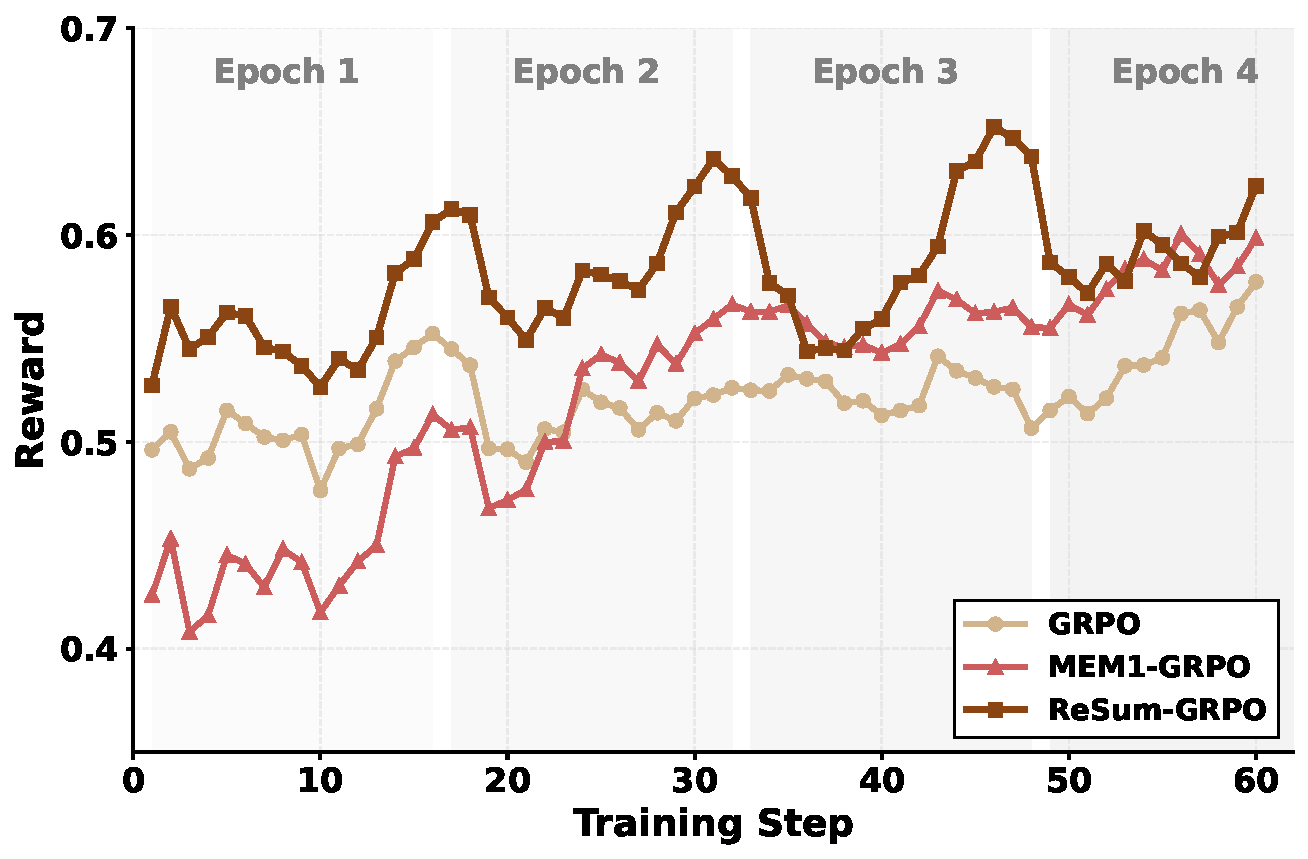
\includegraphics[width=0.42\textwidth]{images/websailor_30b_reward_full.pdf}
    \vspace*{-8pt}
    \caption{\textbf{Training dynamics comparison between GRPO, MEM1-GRPO, and ReSum-GRPO using WebSailor-30B.} ReSum-GRPO generally achieves higher rewards. }
    \label{fig:websailor-30b-reward}
    \vspace*{-8pt}
\end{figure}


\textbf{Overall Evaluation:} In Table~\ref{tab:rl_performance}, we evaluate these RL-trained agents on their respective paradigms and compare them against powerful open-sourced agents, most of which are trained on \textbf{10K+} samples. We can conclude that: 

\textbf{ReSum-GRPO is essential for mastering the ReSum paradigm.} ReSum-GRPO yields significant gains across benchmarks, e.g., WebSailor-3B improves Pass@1 from 8.2\% to 20.5\% on BrowseComp-zh. In contrast, GRPO fails to enable agents to master summary-conditioned reasoning. While standard GRPO enhances ReAct inference, it fails to transfer these benefits to the ReSum paradigm, underscoring the necessity of paradigm-specific optimization.

\textbf{ReSum-GRPO achieves competitive performance with high data efficiency.} Despite using only 1K training samples, ReSum-GRPO enables agents to rival powerful open-source models trained on 10K+ samples. For example, WebSailor-30B achieves 33.3\% on BrowseComp-zh, surpassing ASearcher-32B (15.6\%)~\citep{gao2025asearcher}, MiroThinker-32B (17.0\%)~\citep{miromind2025mirothinker} and WebExplorer-8B (32.0\%)~\citep{liu2025webexplorer}.

\textbf{ReSum offers a balance between performance and efficiency compared to MEM1.} While MEM1-GRPO achieves the highest Pass@1 on BrowseComp, this marginal gain comes at a prohibitive computational cost. As detailed in Appendix~\ref{appendix:mem1_cost}, MEM1-GRPO consumes nearly 3$\times$ more tokens than ReSum for a mere 1.2\% improvement. Consequently, ReSum presents a more practical solution for real-world deployment, maintaining high performance without the excessive overhead of iterative reasoning.

\textbf{Fine-grained Analysis (Appendix~\ref{appendix:fine_grained_resumgrpo}):} For \textbf{training efficiency}, ReSum-GRPO incurs higher computational costs because it prevents the premature truncation of long trajectories. By periodically invoking the summary tool, it allows the agent to learn from extended reasoning trajectories that are typically terminated in standard GRPO. As detailed in Table~\ref{tab:rl_training_time}, this results in approximately 1.5$\times$ training time, a manageable overhead justified by the performance gains. Regarding \textbf{inference efficiency}, we compare performance against resource consumption. As shown in Figures~\ref{fig:token_comp_3mode} and~\ref{fig:toolcall_3mode} in Appendix, ReSum paradigms achieve superior performance with reasonable resource utilization. Finally, our \textbf{qualitative analysis} in Appendix~\ref{appendix:case} reveals that ReSum-GRPO instills an adaptive reasoning strategy. Case studies demonstrate that the agent flexibly switches behaviors: it directly solves simpler queries without summarization while correctly leveraging summaries for complex, long-horizon tasks. This demonstrates that the model masters the ReSum paradigm without losing its proficiency in the ReAct paradigm on simpler tasks.


\subsection{Applicability to Agents with Extensive Context} 

\begin{table}[!t]
    \centering
    \caption{\textbf{Performance comparison between ReAct and Resum using Tongyi-DeepResearch-30B-A3B~\citep{tongyidr} across varying context limits.}}
    \vspace*{-6pt}
    \resizebox{\linewidth}{!}{
    \begin{tabular}{cc|c|cc|cc}
       \toprule
       \rowcolor{COLOR_MEAN}  & & & \multicolumn{2}{c}{\textbf{BrowseComp-zh}} & \multicolumn{2}{|c}{\textbf{BrowseComp}} \\
       \rowcolor{COLOR_MEAN} \multirow{-2}{*}{\begin{tabular}{c} \textbf{Context} \\ \textbf{Limit}
       \end{tabular}} & \multirow{-2}{*}{\begin{tabular}{c} \textbf{Tool} \\ \textbf{Call}
       \end{tabular}} & \multirow{-2}{*}{\textbf{Paradigm}} & Pass@1 &  Pass@3 & Pass@1 &  Pass@3 \\ \midrule

       \multirow{2}{*}{$32k$} & \multirow{2}{*}{40} & ReAct & {41.2} & {57.4} & {27.7} & {43.1} \\ 
       & & \cellcolor{red!10} \textbf{ReSum} & \cellcolor{red!10} \textbf{43.8} & \cellcolor{red!10} \textbf{62.3} & \cellcolor{red!10}\textbf{34.5} & \cellcolor{red!10}\textbf{53.3} \\ \midrule

        \multirow{2}{*}{$48k$} & \multirow{2}{*}{60} & ReAct & {42.5} & {58.5} & {32.8} & {48.7} \\ 
       & & \cellcolor{red!10}\textbf{ReSum} & \cellcolor{red!10}\textbf{46.7} & \cellcolor{red!10}\textbf{62.6} & \cellcolor{red!10}\textbf{38.2} & \cellcolor{red!10}\textbf{54.5} \\ \midrule
       
       \multirow{2}{*}{$64k$} & \multirow{2}{*}{80} & ReAct & 43.6 & 60.9 & 36.3 & 52.4 \\ 
       & & \cellcolor{red!10}\textbf{ReSum} & \cellcolor{red!10}\textbf{48.6} & \cellcolor{red!10}\textbf{66.1} & \cellcolor{red!10}\textbf{40.3} & \cellcolor{red!10}\textbf{57.8} \\  \midrule 

        \multirow{2}{*}{$96k$} & \multirow{2}{*}{100} & ReAct & {46.0} & {62.3} & {39.8} & {56.5} \\ 
       & & \cellcolor{red!10}\textbf{ReSum} & \cellcolor{red!10}\textbf{47.9} & \cellcolor{red!10}\textbf{66.4} & \cellcolor{red!10}\textbf{41.0} & \cellcolor{red!10}\textbf{57.0} \\ \midrule

       \multirow{2}{*}{$128k$} & \multirow{2}{*}{120} & ReAct & 45.7 & 62.3 & 42.2 & 59.2 \\ 
        & & \cellcolor{red!10}\textbf{ReSum} & \cellcolor{red!10}\textbf{46.6} & \cellcolor{red!10}\textbf{62.6} & \cellcolor{red!10}\textbf{44.5} & \cellcolor{red!10}\textbf{59.5} \\ 
       
       \bottomrule
    \end{tabular}
    }
    \label{tab:tongyidr_resum}
    \vspace*{-10pt}
\end{table}


To demonstrate ReSum’s scalability to agents with extensive context, we apply it to the powerful open-source agent, Tongyi-DeepResearch-30B-A3B~\cite{tongyidr}, which supports context windows up to 128$k$. We evaluate performance across five context thresholds with proportionally scaled tool-calling budgets. Under these settings, ReAct is forced to prematurely terminate upon reaching the context limit, whereas ReSum invokes ReSumTool-30B to compress history and sustain the reasoning trajectory.

As shown in Table~\ref{tab:tongyidr_resum}, ReSum consistently outperforms ReAct across all context configurations. The gains are particularly substantial under stricter context constraints, highlighting the benefit of extended exploration. Notably, even with a massive 128$k$ context, ReSum yields improvements. This shows that complex information-seeking tasks demand exploration horizons beyond current context limits and that intelligent summarization remains effective for tackling such challenges.
